\chapter{Einleitung}
\label{ch:einleitung}

\section{Motivation/Aufgabe}

Ziel des Versuchs ist die experimentelle Bestimmung des Planck'schen Wirkungsquantums $h$. Hierfür werden einzelne Spektrallinien des Quecksilberspektrums mit einem Prismenspektrometer aufgespalten und die Energie der durch den Fotoeffekt emittierten Elektronen über die Gegenfeldmethode gemessen. Aus den Sperrspannungen $U_S$, bei denen kein Strom mehr fließt, lässt sich $h$ als Steigung der linearen Beziehung zwischen Sperrspannung und Lichtfrequenz bestimmen. Der Versuch demonstriert damit die Quantennatur des Lichts.

\section{Physikalische Grundlagen}

\subsection{Elektronen in Metallen}

Metalle bestehen aus positiv geladenen Atomrümpfen und delokalisierten Valenzelektronen, den Leitungselektronen. Diese sind innerhalb des Metalls nahezu frei beweglich, können aber das Metallgitter nur verlassen, wenn eine Mindestenergie, die Austrittsarbeit $A$, überwunden wird. Die Energieverteilung der Elektronen folgt der Fermiverteilung. Bei $T=0\,\text{K}$ sind alle Zustände bis zur Fermienergie $E_F$ besetzt, darüber hinaus nicht. Bei $T>0\,\text{K}$ verschwimmt diese Kante und es existieren Elektronen mit Energien $E>E_F$.
\begin{figure}[t!]
    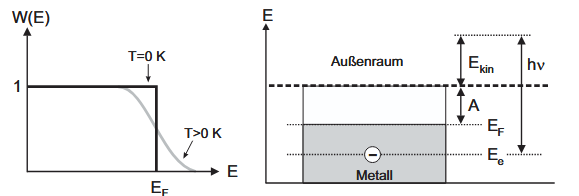
\includegraphics[width=0.45\textwidth]{img/35/einm.png}
    \caption{a) Energieverteilung der Elektronen eines Metalls. b) Potenzialtopfmodell.}
    \label{fig:v}
\end{figure}
\subsection{Der Fotoeffekt}

Trifft ein Photon mit Energie
\begin{equation}
\label{eq:photonenenergie}
E_\text{ph} = h f
\end{equation}
auf ein Elektron der Energie $E_e$, kann dieses aus dem Metall ausgelöst werden. Nach dem Energieerhaltungssatz gilt:
\begin{equation}
\label{eq:einstein}
h f = A + (E_F - E_e) + E_\text{kin}
\end{equation}
Für Elektronen an der Fermikante ($E_e = E_F$) ergibt sich die maximale kinetische Energie:
\begin{equation}
\label{eq:maxEkin}
E_\text{kin,max} = h f - A
\end{equation}

\subsection{Die Gegenfeldmethode}

Die Fotozelle besteht aus einer Metallkathode und einer Anode, zwischen denen eine Spannung $U$ angelegt wird. Bei negativem Potential werden Elektronen mit zu geringer Energie von der Anode ferngehalten. Der Fotostrom $I$ folgt für den linearen Bereich der Kennlinie näherungsweise der Beziehung
\begin{equation}
\label{eq:stromspannung}
I \propto U^2.
\end{equation}
Die Sperrspannung $U_S$ wird durch
\begin{equation}
\label{eq:sperrspannung}
e U_S = h f - A \quad \Rightarrow \quad U_S = \frac{h}{e} f - \frac{A}{e}
\end{equation}
bestimmt. Die Messung für verschiedene Frequenzen ermöglicht die Bestimmung von $h$ als Steigung einer linearen Ausgleichsgeraden.

